\documentclass[conference]{IEEEtran}
%\IEEEoverridecommandlockouts
% The preceding line is only needed to identify funding in the first footnote. If that is unneeded, please comment it out.
\usepackage{cite}
\usepackage{amsmath,amssymb,amsfonts}
\usepackage{algorithmic}
\usepackage{graphicx}
\usepackage{textcomp}
\usepackage{xcolor}
\def\BibTeX{{\rm B\kern-.05em{\sc i\kern-.025em b}\kern-.08em
    T\kern-.1667em\lower.7ex\hbox{E}\kern-.125emX}}

%\usepackage[parfill]{parskip}


\setlength{\parindent}{0pt}
\newcommand{\forceindent}{\leavevmode{\parindent=1em\indent}}

%\usepackage{indentfirst}

\usepackage[hyphens]{url}

%\usepackage[hyphenbreaks]{breakurl}

\def\IEEEkeywordsname{Keywords}

\begin{document}

\title{Differences between Embedded System Operating Systems and Mobile Operating Systems\\
%{\footnotesize \textsuperscript{*}Note: Sub-titles are not captured in Xplore and
%should not be used}
%\thanks{Identify applicable funding agency here. If none, delete this.}
}


\author{\IEEEauthorblockN{Wesly Yii}
\IEEEauthorblockA{\textit{BSc (Hons) in Computer Science} \\
%https://university.sunway.edu.my/tech/bsc-comp-sc
\textit{Sunway University}\\
Selangor, Malaysia\\
18066233@imail.sunway.edu.my}
\and
\IEEEauthorblockN{Tan Chun Ze}
\IEEEauthorblockA{\textit{Bachelor of Software Engineering (Hons)} \\
%https://university.sunway.edu.my/tech/bsc-software-eng
\textit{Sunway University}\\
Selangor, Malaysia\\
15020605@imail.sunway.edu.my}
\and
\IEEEauthorblockN{Lee Ming Zhen}
\IEEEauthorblockA{\textit{Bachelor of Software Engineering (Hons)} \\
\textit{Sunway University}\\
Selangor, Malaysia\\
18088757@imail.sunway.edu.my}
\and
\IEEEauthorblockN{Ryan Aung Yi Yang}
\IEEEauthorblockA{\textit{BSc (Hons) Computer Networking and Security} \\
%https://university.sunway.edu.my/tech/bsc-network-security
%course name too long so truncated some part of it
\textit{Sunway University}\\
Selangor, Malaysia\\
18007906@imail.sunway.edu.my}
}


\maketitle

\forceindent \begin{abstract}
Operating systems play a significant role in powering devices worldwide, this document seeks to provide a comparison between embedded system operating systems and mobile operating systems.
\end{abstract}
\mbox{} \\
\forceindent \begin{IEEEkeywords}
embedded systems, mobile operating systems, operating systems, difference, compare
\end{IEEEkeywords}

\section{Introduction}
\forceindent Human activity is increasingly augmented with computing systems, and the hardware they run on usually have an operating system on it, be it the phones in our pockets that use a mobile operating system, or the subway turnstile that uses an embedded system operating system, they are one of the pieces of software that the general public would not usually think about, yet play a critical role in our modern day lifestyle.

\smallskip
\forceindent In this document, we seek to provide a glimpse into the world of these two types of operating systems, by talking about each of their relevance, usage scenarios, pros and cons.

\smallskip
\forceindent Readers of this document can be expected to briefly understand what mobile OS and embedded system OS respectively are, and how do they compare on various aspects, serving as a first exposure reading material into the world of operating systems.

%TODO: kernel comparison content is removed, update accordingly

\section{Background}
\subsection{Embedded System Operating Systems}

\paragraph{What is it about?}\mbox{} \\
\forceindent Embedded system operating system is a type of operating system that carries out distinct processes for particular devices in order for them to operate optimally. It is just like a toned down version of a standard computer OS with limited functionality\cite{TNEOS}.
Embedded system operating systems may exist as a standalone independent system or belong as a part of something bigger. There are five types of embedded operating system; Multi-Tasking Operating System, Rate Monotonic Operating System, Preemptive Operating System, Single System Control Loop and Real Time Operating System. Generally, Its main focus is to let a certain device function as intended by running its codes
\cite{ITEOSMC}. \\

\\
\paragraph{Why the need for it?}\mbox{} \\
\forceindent Embedded systems operating systems are everywhere nowadays. The main reasons for embedded OS to exist is to act as a partitioning tool as well as manage hardware and software resources for the embedded system to work as intended. It also helps to simplify the steps of developing softwares in the upper layer by providing an abstraction layer.  Other than that,there is a need for it as it is able to fill in a niche in our lives. The need for it lies in how embedded operating systems can perform a dedicated function for a specific device to run while also allow it to be less demanding in terms of resource consumption. Devices such as cameras, medical equipment, household appliances all require an embedded operating system to work. Some of it are also designed to be able to withstand harsh temperatures and environments in which other operating systems will fail\cite{TNEOS}.
%\forceindent Mobile OS is originally derived from the computer OS which was then evolved into an embedded OS and then to the present smartphone-oriented OS. Throughout the evolutions, the architecture of mobile OS has become simpler compared to the previous versions. In terms of hardware, the factor size of microprocessors and peripherals has been reduced to accommodate the modern design of smartphones.

%\smallskip
%\forceindent Technically, smartphones do not require an operating system and the device can just run without problem but it would be a mess since there will be no operating system present to manage the memory, storage and applications. Therefore, the main reason for embedded OS to exist is to act as a partitioning tool as well as manage hardware and software resources for the embedded system to work as intended. It also simplifies software development in the upper layer by providing an abstraction layer. The need for it lies in how embedded operating systems can perform a dedicated function for a specific device to run while also allow it to be less demanding in terms of resource consumption\cite{ITEOSPV}.
%\\
\medskip
\paragraph{What is the application?}\mbox{} \\
\forceindent Applications of embedded system OS include Embedded Linux, iOS, Windows Mobile OS, Blackberry OS, and Symbian. A Linux operating system that is utilized within embedded devices and appliances is called Embedded Linux. ATM machines utilising Windows XP is also an application of embedded operating systems.

\subsection{Mobile Operating Systems}\\
\paragraph{What is it about?}\mbox{} \\
\forceindent A mobile OS is another type of operating system that is created for the sole purpose of powering mobile devices. These mobile devices include PDAs, tablets, smartphones etc. Similar to how the Windows operating system works in a desktop, a mobile operating system allows different kinds of applications to run on a mobile device by serving as a software platform beneath the apps. All the features and functions that are available on mobile devices are all set by the corresponding mobile operating system. On top of that, mobile operating systems will also be in control of the third-party programs that are used on the mobile device.
\medskip
\\
\paragraph{Why the need for it?}\mbox{} \\
\forceindent Mobile OS is originally derived from the computer OS which was then evolved into an embedded OS and then to the present smartphone-oriented OS. Throughout the evolutions, the architecture of mobile OS has become simpler compared to the previous versions. In terms of hardware, the factor size of microprocessors and peripherals has been reduced to accommodate the modern design of smartphones.

\medskip
\forceindent Technically, smartphones do not require an operating system and the device can just run without problem but it would be a mess since there will be no operating system present to manage the memory, storage and applications. Therefore, a mobile operating system is essential for mobile devices to run ideally. A mobile operating system would enable multitasking, which means that multiple applications can run at one time. It will also allow the users to adjust the brightness and volume of all the applications through a single button. Other than that, applications would then be compatible and portable across multiple devices of different brands.

%\forceindent A mobile operating system is essential for mobile devices to run ideally. A mobile operating system would enable multitasking, which means that multiple applications can run at one time. It will also allow the users to adjust the brightness and volume of all the applications through a single button. Other than that, applications would then be compatible and portable across multiple devices of different brands.
\\
\medskip
\paragraph{What is the application?}\mbox{} \\
\forceindent Some notable examples of mobile OS are Apple’s iOS and Google’s Android OS. The differences between iOS and Android is that iOS is designed to only run on Apple devices within its XNU kernel while Android is an open source software which implies that it can be used by other mobile device manufacturers who are then able to customize the Android source code to fit their own device’s needs. Apple has also released other mobile OS meant for their Apple watch and iPad which is watchOS and iPadOS respectively\cite{CSMOS}.


\smallskip
\forceindent Covering all types of operating systems in embedded systems and mobile systems can be vague and challenging. With that said, Operating  systems  that are ubiquitous will be chosen to elaborate more in depth about their structure and features.


%\bigskip
\medskip
\section{In-depth review and discussion}

\subsection{Major differences between Microkernel and Monolithic Kernel}
\paragraph{Address space and size}\mbox{} \\
\forceindent In Microkernel, Other services are implemented as user-level programs located in separate address space from kernel mode\cite{Galvinbook}. In the Monolithic kernel, Fundamental OS services and other non-essential services are combined together into one single address space\cite{Galvinbook}.  In terms of size, Microkernel only provides fundamental OS services such as interprocess communication(IPC), memory management and CPU scheduling\cite{Galvinbook}. Therefore the size of the microkernel is smaller than the Monolithic kernel because the Monolithic kernel combined other services with essential services in the same address space as mentioned before.

\bigskip
\paragraph{Communication between software and hardware}\mbox{} \\
\forceindent Interprocess communication in Microkernel uses message passing\cite{Burger} allowing other services to exchange messages between each other indirectly.

\bigskip
\paragraph{Extensibility}\mbox{} \\
\forceindent Different approaches on address space influence the extensibility of the kernel, separated address space used by the Microkernel can easily add new services. However, the Monolithic kernel is required to recompile the whole kernel for adding new services or features\cite{educba}. In the Monolithic kernel, system call is used to allow application programs to interact with the kernel.

%\paragraph{Microkernel in QNX Architecture} \mbox{} \\
\medskip
\subsection{Microkernel in QNX Architecture}
According to \cite{embhack}, QNX is the most famous operating system used in real-time embedded systems. QNX  heavily relies on Microkernel architecture to support its own operating system\cite{Galvinbook}\cite{Burger}.
%\forceindent QNX is one of the operating systems used in real-time embedded systems. QNX heavily relies on Microkernel architecture to support its own operating system\cite{Burger}\cite{Galvinbook}.
%TODO: yet add page number for Galvinbook
%\subsection{QNX operating system}

\begin{figure}[h]
\caption{QNX Microkernel model}
\begin{center}
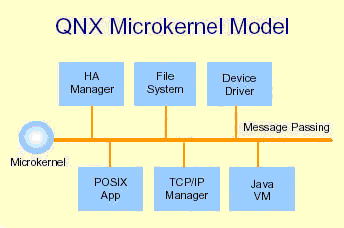
\includegraphics[scale=0.5]{./images/QNX_microkernel_mode.png}
\end{center}
\end{figure}

\forceindent Figure 1 shows QNX added features in the user space address on top of the microkernel. QNX utilizes synchronous message passing allowing services to communicate and synchronize better\cite{Burger} with other services.

%\paragraph{}
%\forceindent Microkernel only provides fundamental OS services including interprocess communication(IPC), memory management and CPU scheduling\cite{Galvinbook}. Other services are implemented as user-level programs located in separate address space from Microkernel\cite{Galvinbook}. To achieve extensible service implementation and communication between other services and microkernels. IPC is an important function as it uses message passing\cite{Burger} allowing other services to exchange messages between each other indirectly.

\medskip
%\paragraph{Linux kernel in Android architecture} \mbox{} \\
\subsection{Linux kernel in Android architecture}
\forceindent Android OS has a 86.1\% market share in the mobile OS market \cite{SMS}. It is based on the Linux kernel with a monolithic structure.

\begin{figure}[h]
  \caption{Android architecture}
\begin{center}
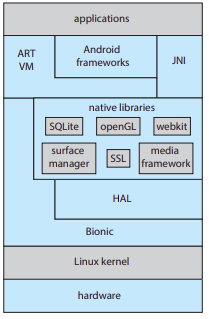
\includegraphics[scale=0.7]{./images/Android_architecture.png}
\end{center}
\end{figure}

%[1] again ffs, assume it is [A] so it Galvinbook
\smallskip
%\forceindent Fundamental OS services and other non-essential services are combined together into one single address space\cite{Galvinbook}, and system calls are used in android architect to allow application programs to interact with the kernel\cite{TDDBM}.

\smallskip
\forceindent Figure 2 indicates that android’s architecture consists of a layered stack of software providing an abundance set of frameworks and libraries to support crucial hardware features including graphics, audio\cite{Galvinbook}. For that reason, it gives the android operating system to be compatible with any types of android enabled devices.

\smallskip
\forceindent With the accumulated resources gathered, it can be concluded that embedded OS and mobile OS use different approaches on OS structure for different benefits, and using the wrong OS type could be devastating. Thus, the pros and cons of embedded operating system and mobile operating system shall be explained to aid the choosing of OS architectures.

%\bigskip
\medskip
\subsection{Pros of Embedded OS}
\paragraph{Loads faster and consumes less power} \mbox{} \\
\forceindent Embedded system OS can be attached to a PC and will always load faster from the flash compared to a standard computer OS because of the limited features built in it. This is beneficial when users only need to perform a single task such as browsing the internet\cite{TDDBM}.

\medskip
\paragraph{Distinct functions} \mbox{} \\
\forceindent Embedded system OS differs greatly from standard OS in terms of their abilities to perform different functions. Embedded OS will be limited to one single task and will perform the task regardless of user intervention. Examples of devices using an embedded OS would range from a simple toaster to specific embedded systems such as the QNX4 RIOS\cite{NOSvsEOS}.

\medskip
\subsection{Cons of Embedded OS}
\paragraph{Hardly Scalable} \mbox{} \\
\forceindent Embedded system OS are usually not upgradable since it's system stays fixed after the initial configuration. Some embedded systems OS like the ones in  ATM machines are also designed to not receive upgrades to prevent tampering. Embedded system OS only allows upgrades if the chip is flashable. An example of an upgradable embedded system OS would be the one in a wifi router, it can be updated by flashing the card in the router upon downloading the new firmware\cite{lifewire}.

\medskip
\subsection{Pros of Mobile OS}
\paragraph{Open source platforms are constantly updated and well-supported} \mbox{} \\
\forceindent Mobile OS such as Android open source software is one of the most widely used Mobile OS in the world. It is utilised by top mobile conglomerates like Huawei and Samsung. In recent years, we could see that there are more variations of the open source platform to support and cater to specific markets like the HongMengOS (Harmony OS) that is launched in 2019 for new Huawei devices exclusively\cite{HuaweiHongmeng}. Such new launches suggest that Mobile OS are still in high demand and will be the focal point of operating systems in many years to come.

\medskip
\paragraph{Convenience and flexibility} \mbox{} \\
\forceindent Mobile OS is a newer concept and is built to focus on being convenient to its users. It is improved on existing OS and opts to strive in responsive design, consistent and stable network access and possible improvements to be used in the diverse wireless environment\cite{technopedia}.

\smallskip
\forceindent Mobile OSs like Android are open-source and are widely used as a base for many relatable OS like HarmonyOS. The fact that it is open source opens itself to many possibilities. It is flexible because many others improve and adjust the software to cater to their own needs.

\medskip
\paragraph{Scalability and maintainability}\mbox{} \\
\forceindent Mobile OS outcompetes embedded OS in this regard by a wide margin. They are built to handle any number of connections from the user side, handling errors and backend API interactions\cite{mediumScalability}. The maintainability instead is a way to iterate and improve upon existing software and OS efficiently when it comes to debugging and further improvements.\\

\subsection{Cons of Mobile OS}
\paragraph{Instability} \mbox{} \\
\forceindent Mobile OS struggles with the constraints of handling constant cellular interruptions and communications, power issues and the load on handling multiple applications launched by the user\cite{AAWP}. On average, a mobile phone easily uses anywhere from 50 to 500 processes on a comparatively smaller capacity compared to an embedded system OS which commonly runs a single shell. This leads to frequent crashes and bugs that leads to complications and instabilities.

\medskip
\paragraph{Battery / Power} \mbox{} \\
\forceindent Mobile OS runs on a limited battery capacity unlike embedded OS which runs with a constant power supply. Although modern mobile devices now are equipped with better batteries, they are still lacking and unable to keep up with improvements in graphics and animations like in triple A games for mobiles. Many background processes are also capable of draining the battery, accelerating its wear.

\section{Conclusion}
\forceindent After looking into both embedded system OS and mobile OS, we can see that both types of OS have their own pros and cons. However, in terms of efficiency in performing what they are meant to do, QNX microkernel architecture is by far the most superior. Being small in size, it provides complete memory protection as it runs in the kernel space while other processes run in the user space. Most importantly, we think QNX is a good fit here as it is the best for mission critical applications due to the fact it never crashes thus making it robust, as any third party crashes does not impact the kernel itself and it keeps running at all times\cite{quora}.
%\vfill

%\section*{Acknowledgment}
%The preferred spelling of the word ``acknowledgment'' in America is without 
%an ``e'' after the ``g''. Avoid the stilted expression ``one of us (R. B. 
%G.) thanks $\ldots$''. Instead, try ``R. B. G. thanks$\ldots$''. Put sponsor 
%acknowledgments in the unnumbered footnote on the first page.

\bibliographystyle{IEEEtran}
\bibliography{mainbib}

\end{document}
